%%%%%%%%%%%%%%%%%%%%%%%%%%%%%%%%%%%%%%%%%
% University Assignment Title Page 
% LaTeX Template
% Version 1.0 (27/12/12)
%
% This template has been downloaded from:
% http://www.LaTeXTemplates.com
%
% Original author:
% WikiBooks (http://en.wikibooks.org/wiki/LaTeX/Title_Creation)
%
% License:
% CC BY-NC-SA 3.0 (http://creativecommons.org/licenses/by-nc-sa/3.0/)
% 
% Modified for COSC343 by:
% Lech Szymanski (5/5/20)

\documentclass[12pt]{article}
\usepackage{cosc343style}


% Paper code for COSC343
\papercode{COSC343}

% Your project title (change appropriately for the assignment)
\title{Assignment X report}

% Your name
\author{John \textsc{Smith}}
\studentid{555555}


% Date, change the \today to a set date if you want to be precise
\reportdate{\today}

\begin{document}


\maketitle


\section{Introduction}

Introduce the assignment and what it is about.  For example, the purpose of this document is to provide a template for your report with examples of commonly used \LaTeX{} commands and features.  You don't need to repeat all the details of the information provided in the assignment description.  The purpose of this is just to provide some context for everything that follows.   

\section{Main body}

You probably don't want to call this section "Main body"...but it's essentially what you need to do next --  report on the work you've done for your assignment: the approach, results, analysis, and anything else that was asked for in the assignment specification.  

You can use section and subsection commands to organise your document - either break the main body into multiple sections, or have it as a one section with subsections.   \LaTeX{} handles all the formatting and numbering automatically. Use ref and label commands for cross-references.  

\subsection{Citing}

You might want to cite some sources of your information.  For instance, a reference for \LaTeX{} can be found here \cite{latexcompanion}.

\subsection{How to compile \LaTeX{}}

\LaTeX{} documents are prepared using markup language and need to be compiled to produce pdfs.  

The easiest way is to use the \href{https://www.overleaf.com}{Overleaf service} - it's free for private projects.  Create an account and once you login you can create different projects (essentially different documents).  After clicking on "New Project" select "Upload" project and upload the cosc343report.zip file where this file came from.  The template will open on the website and you'll be able to write your report through Browser, compiling LaTeX online and have it saved on remote server.  Later you just download the final pdf and submit with your code.    

Alternately, you can install LaTeX compiler on your machine and compile .tex file yourself.  On a macOS you need to download and install \href{http://www.tug.org/mactex/downloading.html}{MacTeX}.  Then, using a program like \href{http://pages.uoregon.edu/koch/texshop/}{TexShop} (free), or \href{https://www.texpad.com/}{Texpad} (awesome, but not free) you can edit and compile a .tex file into the .pdf.


\subsection{Tables and Figures}

Use the table and tabular commands for basic tables --- see Table~\ref{tab:widgets}, for example. You can include a figure (JPEG, PNG or PDF) with the \verb$\includegraphics$ command as in the code for Figure~\ref{fig:frog} below.

% Commands to include a figure:
\begin{figure}
\centering
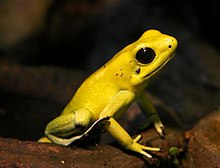
\includegraphics[width=0.4\textwidth]{figures/frog.jpg}
\caption{\label{fig:frog}This is a figure caption.}
\end{figure}

\begin{table}
\centering
\begin{tabular}{l|r}
Item & Quantity \\\hline
Widgets & 42 \\
Gadgets & 13
\end{tabular}
\caption{\label{tab:widgets}An example table.}
\end{table}

\subsection{Mathematics}

\LaTeX{} is great at typesetting mathematics. Let $X_1, X_2, \ldots, X_n$ be a sequence of independent and identically distributed random variables with $\text{E}[X_i] = \mu$ and $\text{Var}[X_i] = \sigma^2 < \infty$, and let
$$S_n = \frac{X_1 + X_2 + \cdots + X_n}{n}
      = \frac{1}{n}\sum_{i}^{n} X_i$$
denote their mean. Then as $n$ approaches infinity, the random variables $\sqrt{n}(S_n - \mu)$ converge in distribution to a normal $\mathcal{N}(0, \sigma^2)$.

\subsection{Lists}

You can make lists with automatic numbering \dots

\begin{enumerate}
\item Like this,
\item and this
\end{enumerate}
\dots or bullet points \dots
\begin{itemize}
\item Like this,
\item and this
\end{itemize}

\section{Conclusion}

Concluding remarks.  It could be a brief summary and/or comments on what you have learned/enjoyed/struggled with.      Depending on the space taken up by figures and formatting the report (excluding the Appendix) should be somewhere in the range of 3-5 pages.  Remember, it's not about creative space-wasting to hit the 4 pages, but about reporting on your work and results, so I can tell how much you have done and learned.  


%The environment \thebibliography produces a list of references; such list will be titled "References". A parameter inside braces, 3 in the example, indicates the number of entries to be added; this parameter can not be greater than 99.

%To create a bibliography entry the command \bibitem is used. A parameter inside braces is set to label this entry and can later be used as identifier for this reference. After the closing brace the text with the name of the author, the book title, publisher and so on is entered. 

%Any choice of citation style is acceptable as long as you are consistent.

\begin{thebibliography}{3}

\bibitem{latexcompanion} 
Michel Goossens, Frank Mittelbach, and Alexander Samarin. \textit{The \LaTeX\ Companion}. Addison-Wesley, Reading, Massachusetts, 1993.

\end{thebibliography}


% Activate the appendix
% from now on sections are numerated with capital letters
\appendix

\renewcommand{\thesection}{Appendix \Alph{section}}

\section{Some extra things}

If you have anything more to add you might want to add it to the appendix.  The could be some not details, that could be distracting from the main points in the main text, but are still important to mention.  You don't need to have an appendix if you don't think you need one.

\textbf{Do not stick code in the appendix} - any code should be submitted as a separate file (.py file for Python code).  


\end{document}